\documentclass{beamer}
\usepackage[utf8x]{inputenc}
\usepackage[ngerman]{babel}
\usepackage{multimedia}
\usepackage{hyperref}
\usepackage{graphicx}
\usetheme[compress]{Berlin}
\title[]{Einführung in die Android App Entwicklung}
\author{Philipp Deppenwiese}
\institute{https://github.com/zaolin/android-app-demo}
\date{\today}
\begin{document}

\begin{frame}
\titlepage
\end{frame}

\begin{frame}{Das Labor e.V.}
\begin{block}{Bochums Hackerspace}
"Wir schaffen mit Technik Faszinierendes und Nützliches."
\end{block}
\end{frame}

\begin{frame}{Android}
\begin{figure}[hb]
 \centering
 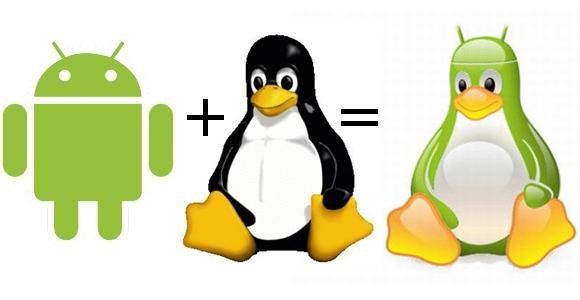
\includegraphics[width=4in]{android-linux}
\end{figure}
\end{frame}

\begin{frame}{Worum es in dem Vortrag nicht geht}
\begin{itemize}
\item Appstore und Zertifizierung
\item Versionskontrolle
\item IDE Funktionalität
\item Einbinden \& Entwicklung von nativen Bibliotheken
\item Reflections
\item Tiefergreifende UI Entwicklung
\item Netzwerk
\item usw..
\end{itemize}
\end{frame}

\begin{frame}{Weiterführend}
\begin{center}
https://developer.android.com/guide/index.html
\end{center}
\end{frame}

\begin{frame}{Roter Faden}
\begin{itemize}
\item API Level
\item App Struktur, Manifest \& Komponenten
\item Framework, Ressourcen \& UI
\item Zugriffsrechte 
\item Inter-Prozess-Kommunikation
\item Native Unterstützung
\item Hardware Einrichten
\item Workshop Part 1
\item Workshop Part 2
\item Workshop Part 3
\end{itemize}
\end{frame}

\begin{frame}
\begin{center}
\huge\textbf{API Level}
\end{center}
\end{frame}

\begin{frame}{API Level}
\begin{itemize}
\item Das Android Framework welches eine Java Bibliothek darstellt besitzt eine Schnittstellen (API) Versionierung.
\item Jede API Version ist von der System version abhängig.
\item Android 5.1 == API Level 22
\item Android 5.0 == API Level 21
\item Android 4.4 == API Level 19
\end{itemize}
\end{frame}

\begin{frame}
\begin{center}
\huge\textbf{App Struktur, Manifest \& Komponenten}
\end{center}
\end{frame}

\begin{frame}{App Struktur}
\begin{itemize}
\item Jede Android App ist eine Zip Datei !
\item Diese enthält unter META-INF die zwei Manifest Dateien und ein PKCS7 Container worin sich Signatur und Zertifikat befinden.
\end{itemize}
\begin{figure}[hb]
 \centering
 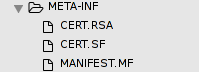
\includegraphics[scale=0.6]{app-contents-1}
\end{figure}
\end{frame}

\begin{frame}{App Struktur}
\begin{itemize}
\item Unter z.B. org. und com. befinden sich weitere App spezifisch Dateien ( Lizenzen, README ).
\item lib enthält Architektur spezifische native Bibliotheken.
\item assets ist ähnlich dem res Ordner enthält jedoch alle möglichen Dateien.
\end{itemize}
\begin{figure}[hb]
 \centering
 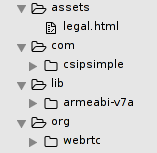
\includegraphics[scale=0.6]{app-contents-3}
\end{figure}
\end{frame}

\begin{frame}{App Struktur}
\begin{itemize}
\item In dem res Ordner finden sich sämtliche Ressourcen die UI spezifische Elemente wie
Strings, Grafiken usw. 
\end{itemize}
\begin{figure}[hb]
 \centering
 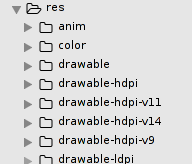
\includegraphics[scale=0.6]{app-contents-2}
\end{figure}
\end{frame}

\begin{frame}{App Struktur}
\begin{itemize}
\item Die AndroidManifest.xml definiert das Android Package Kit.
\item Die resources.arsc ist eine Index Datei der Ressourcen.
\item Die classes.dex enthält alle kompillierten Klassen als DEX Bytecode.
\end{itemize}
\begin{figure}[hb]
 \centering
 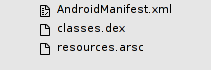
\includegraphics[scale=0.6]{app-contents-4}
\end{figure}
\end{frame}

\begin{frame}{App Manifest}
\begin{itemize}
\item Jedes Android Paket hat einen eindeutigen und einzigartigen Paketnamen !
\item Das Manifest beschreibt alle Komponenten die zum Android Paket dazugehören.
\item Ebenso finden sich hier die Zugriffsrechte die diese App benötigt. Diese werden einem
bei der Installation der App angezeigt.
\item Ebenfalls findet man zusätzliche Metadaten die zum Android Paket gehören.
\end{itemize}
\end{frame}

\begin{frame}{App Manifest}
\begin{figure}[hb]
 \centering
 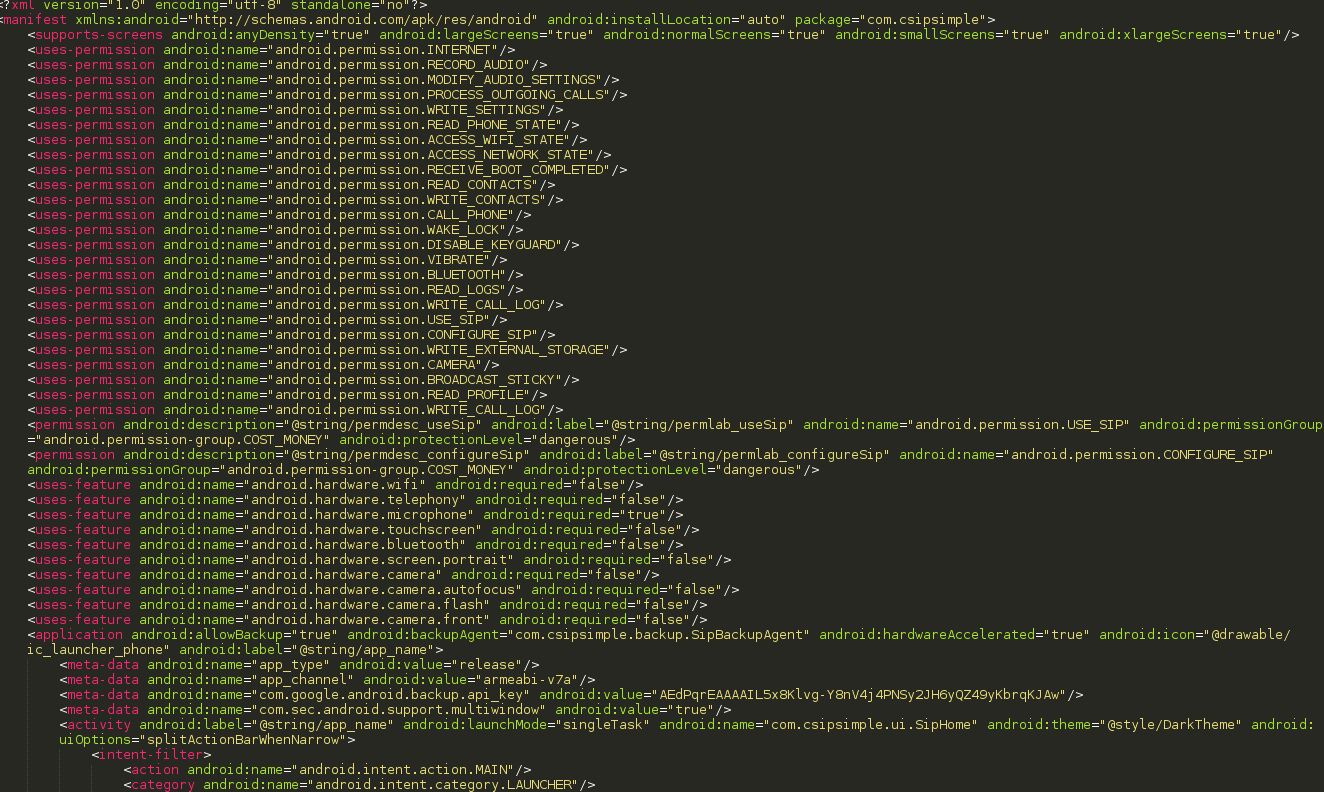
\includegraphics[scale=0.23]{manifest}
\end{figure}
\end{frame}

\begin{frame}{App Komponenten}
\begin{itemize}
\item In der Android Welt existieren mehrere Komponenten die Inhalt einer Applikation sein können.
\item Um eine Komponente verwenden zu können muss von dieser geerbt werden.
\item Mehrere Komponenten können Teil einer Applikation sein.
\end{itemize}
\end{frame}

\begin{frame}{Activity}
\begin{figure}[hb]
 \centering
 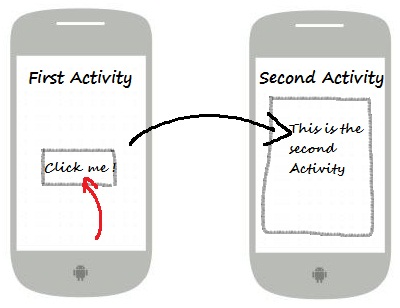
\includegraphics[scale=0.7]{android-activity}
\end{figure}
\end{frame}


\begin{frame}{Activity}
\begin{itemize}
\item Eine Klasse die einen Screen beschreibt in dem ein Benutzer Interaktionen tätigen kann.
\item Diese Klasse besitzt einen Lifecycle wie alle Komponenten und kann durch Intents aufgerufen werden.
\item Beim Start einer Android Applikation wird eine Hauptaktivität gestartet welche den ersten Screen anzeigt von dem aus weitere Activities gestartet werden können.
\end{itemize}
\end{frame}

\begin{frame}{Activity}
\begin{figure}[hb]
 \centering
 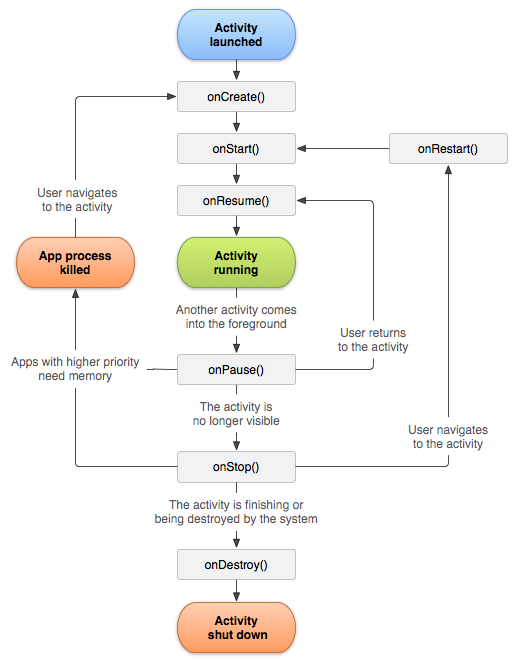
\includegraphics[scale=0.3]{activity-lifecycle}
\end{figure}
\end{frame}

\begin{frame}{Service}
\begin{figure}[hb]
 \centering
 
\includegraphics[scale=0.7]{android-service}
\end{figure}
\end{frame}

\begin{frame}{Service}
\begin{itemize}
\item Eine Service ist ein Hintergrunddienst der auch nach schlafen legen der Activity weiterhin aktiv bleibt.
\item Services werden meistens via Interfaces aufgerufen die sie beim sogenannten ServiceManager registrieren können.
\item Dadurch wird es möglich eine lokale oder auch Inter-Prozess-Kommunikation zwischen App oder Activity zu erstellen.
\item Nebenbei Android selbst bietet eine Menge System Services an ! 
\end{itemize}
\end{frame}

\begin{frame}{BroadcastReceiver}
\begin{figure}[hb]
 \centering
 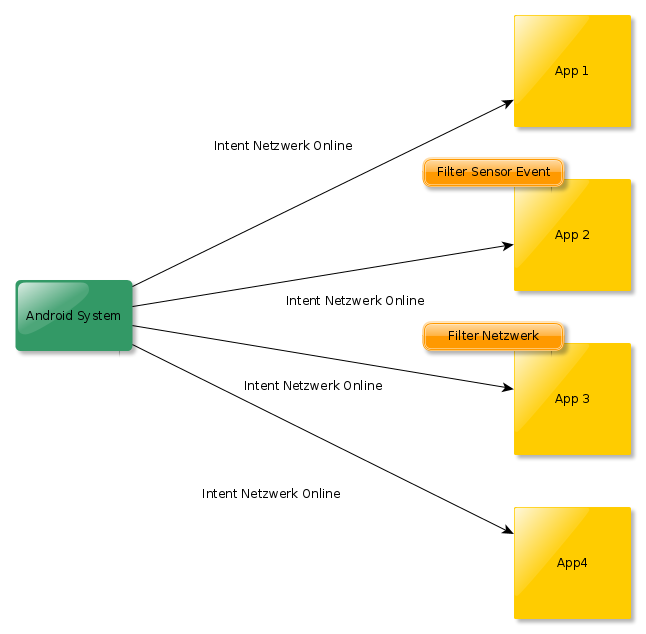
\includegraphics[scale=0.3]{android-br}
\end{figure}
\end{frame}

\begin{frame}{BroadcastReceiver}
\begin{itemize}
\item Diese Klasse funktioniert Event basiert und nutzt den Intent IPC Mechanismus !
\item Es können sämtliche System und App Intents gelesen werden.
\item Jeder Receiver kann ein Filter definieren indem er nur bestimmte Intent Typen zulässt.
\end{itemize}
\end{frame}


\begin{frame}{ContentProvider}
\begin{figure}[hb]
 \centering
 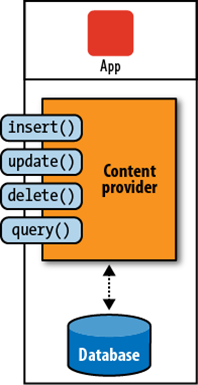
\includegraphics[scale=0.4]{android-cp}
\end{figure}
\end{frame}

\begin{frame}{ContentProvider}
\begin{itemize}
\item Ist eine Art von Service welcher via Datenbanken Informationen abspeichert.
\item Nutzen SQLite als Datenbank Backend.
\end{itemize}
\end{frame}

\begin{frame}
\begin{center}
\huge\textbf{Framework, Ressourcen \& UI}
\end{center}
\end{frame}

\begin{frame}{Android Framework}
\begin{itemize}
\item API level spezifisch.
\item Eine Android Bibliothek die sämtliche Funktionalitäten anbietet.
\item Ist auch Teil des SDK damit man Android Apps entwickeln kann.
\item Diese Bibliothek ist extrem groß und eine offizielle Dokumentation ist im World Wide Web zu finden.
\end{itemize}
\end{frame}

\begin{frame}{Android Ressourcen}
\begin{itemize}
\item Android Ressourcen bestehen aus layout, strings, bilder usw..
\item Ressourcen werden im code durch ID's geladen und können somit Objekten zugewiesen werden.
\item Als primäre benötigt man ein Layout welches unter res/layout zu finden ist.
\item Das einfachste Layout ist das lineare welches wir auch in den Workshops nutzen werden.
\end{itemize}
\end{frame}

\begin{frame}{Android UI}
\begin{figure}[hb]
 \centering
 
\includegraphics[scale=0.6]{android-layout}
\end{figure}
\end{frame}

\begin{frame}{Android UI}
\begin{itemize}
\item Eine Layout besteht aus mehreren Views und auch View Gruppen.
\item Dadurch ist es möglich eine generische Anordnung herzuleiten.
\item Es gibt drei Typen von Layouts: Linear, Relative, List und Grid.
\end{itemize}
\end{frame}

\begin{frame}
\begin{center}
\huge\textbf{Zugriffsrechte}
\end{center}
\end{frame}

\begin{frame}{Android Zugriffsrechte}
\begin{itemize}
\item Android verfügt im Application Layer über ein Capabillity based Access Control.
\item Das heisst jede App die Zugriffsrechte z.B. auf das Netzwerk benötigt muss diese in der
AndroidManifest.xml definieren.
\item Dadurch wird der Nutzer bei der Installation einer Applikation nach den Rechten gefragt.
\item Zugriffsrechte können auch selbst durch die App neu definiert werden die Interfaces beschränken.
\end{itemize}
\end{frame}

\begin{frame}{Android Zugriffsrechte}
\begin{figure}[hb]
 \centering
 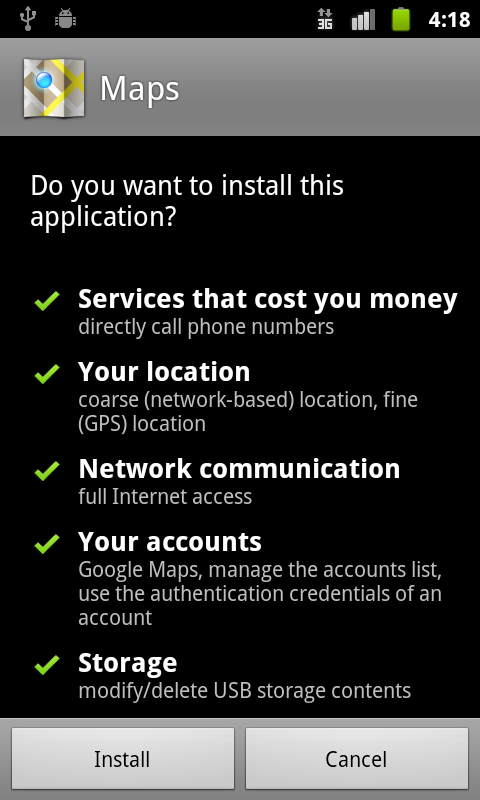
\includegraphics[scale=0.23]{android-perms}
\end{figure}
\end{frame}

\begin{frame}{Android Zugriffsrechte}
\begin{figure}[hb]
 \centering
 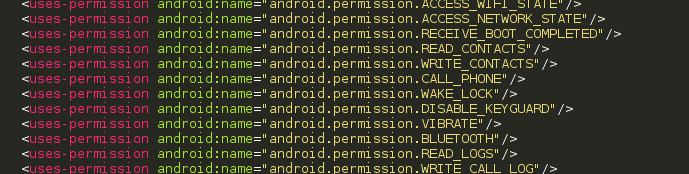
\includegraphics[scale=0.5]{perms-more}
\end{figure}
\end{frame}

\begin{frame}
\begin{center}
\huge\textbf{IPC}
\end{center}
\end{frame}

\begin{frame}{Basis}
\begin{itemize}
\item IPC basiert meist auf Binder IPC.
\item Es existiert ein ServiceManager welche alle Android Services vorhält.
\item Highlevel Netzwerkimplementierung kann auch für IPC benutzt werden.
\end{itemize}
\end{frame}

\begin{frame}{Intents}
\begin{itemize}
\item Die meist genutzte Art zwischen Applikationen zu kommunizieren.
\item Kann nicht nur Informationen sondern auch Daten transportieren.
\item Die Gegenstelle benötigt einen BroadcastReceiver und IntentFilter.
\end{itemize}
\end{frame}

\begin{frame}{Services}
\begin{itemize}
\item Services bieten ein Interface via Binder an (AIDL).
\item Dadurch kann man Methoden im einer Serviceinstanz aufrufen.
\item Services können sich selbst durch die Android Zugriffskontrolle schützen.
\end{itemize}
\end{frame}

\begin{frame}{LocalSockets}
\begin{itemize}
\item Highlevel Netzwerkimplementierung um Sockets nutzen zu können.
\item Apps können via Client-Server Beziehung kommunizieren.
\end{itemize}
\end{frame}

\begin{frame}
\begin{center}
\huge\textbf{Native Unterstützung}
\end{center}
\end{frame}

\begin{frame}{C \& C++ Bibliotheken}
\begin{itemize}
\item Java kann via Java Native Interface C und C++ Bibliotheken laden.
\item Diese müssen mit einer nativen Toolchain auch NDK genannt für die Platform kompiliert werden.
\item Dadurch wird es Funktionen aus Low level Bibliotheken zu nutzen.
\end{itemize}
\end{frame}

\begin{frame}
\begin{center}
\huge\textbf{Ende}
\end{center}
\end{frame}

\begin{frame}
\begin{center}
\huge\textbf{Hardware Einrichten}
\end{center}
\end{frame}

\begin{frame}{Treiber}
\begin{itemize}
\item Unter Windows oder OSX muss man evtl. noch die sogenannten ADB Treiber installieren.
\item Diese sollte man auf der Gerätehersteller Webseite finden können.
\end{itemize}
\end{frame}

\begin{frame}{Debugging Modus}
\begin{itemize}
\item Aktivieren des Debugging Modus ermöglicht es live und realistisch Apps debuggen.
\item App kann auf dem Gerät direkt gestartet werden.
\item Deutlich schneller als der Emulator und stellt eine optimale Testumgebung dar.
\item Zugriff der Nutzung wird durch Bestätigung gewährt.
\end{itemize}
\end{frame}

\begin{frame}{Debugging Modus}
\begin{figure}[hb]
 \centering
 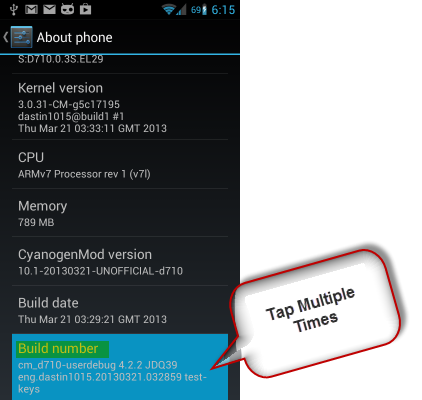
\includegraphics[scale=0.4]{android-build}
\end{figure}
\end{frame}

\begin{frame}{Debugging Modus}
\begin{figure}[hb]
 \centering
 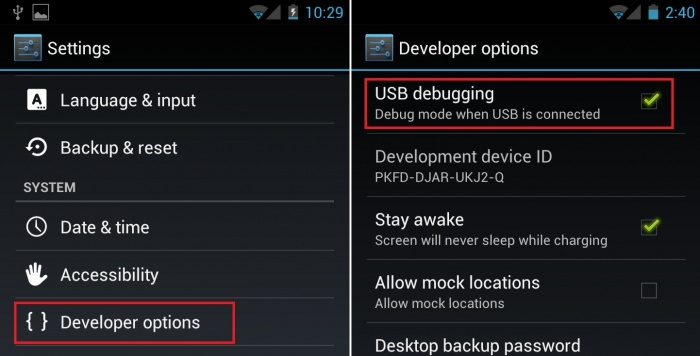
\includegraphics[scale=0.4]{android-debugging}
\end{figure}
\end{frame}

\begin{frame}
\begin{center}
\huge\textbf{Workshop Part 1}
\end{center}
\end{frame}

\begin{frame}
\begin{center}
\huge\textbf{Workshop Part 2}
\end{center}
\end{frame}

\begin{frame}
\begin{center}
\huge\textbf{Workshop Part 3}
\end{center}
\end{frame}

\begin{frame}
\begin{center}
\huge\textbf{Quellen}

www.groovypost.com
www.companionlink.com
www.xda-developers.com
www.tutorialspoint.com
www.pcmag.com
developer.android.com
\end{center}
\end{frame}

\end{document}

